% Diese Zeile bitte -nicht- aendern.
\documentclass[course=erap]{aspdoc}

%%%%%%%%%%%%%%%%%%%%%%%%%%%%%%%%%
\newcommand{\theGroup}{127}
\newcommand{\theNumber}{A219}
\author{Syrine Aidani \and Adem Trabelsi \and Ahmed Mhamdi}
\date{Wintersemester 2023/2024} 
%%%%%%%%%%%%%%%%%%%%%%%%%%%%%%%%%

\title{Gruppe \theGroup{} -- Abgabe zu Aufgabe \theNumber}

\usepackage{graphicx} 
\usepackage{subcaption}
\usepackage{amsthm}
\usepackage{hyperref}
\usepackage{amsmath}
\usepackage{amssymb}
\usepackage[margin=1.5in]{geometry} 
\usepackage[ruled,vlined]{algorithm2e}

\graphicspath{{resources/}}
\renewcommand\proofname{Beweis}
\newcommand{\clamp}[3]{\text{clamp}^{#1} _{#2} (#3)}

\begin{document}
\maketitle


\section{Einleitung}
Der Schwerpunkt dieses Projekts liegt auf der Konvertierung farbiger Bilder in Graustufen und der darauf folgenden Durchführung einer Tonwertkorrektur. Als Eingabe lesen wir zuerst 24bpp PPM (P6) Pixelbilder \cite{netpbm}. Jeder Farbpixel wird als Vektor mit den drei Farbkanälen Rot R, Grün G und Blau B definiert. Durch die Berechnung eines gewichteten Durchschnitts D, wandeln wir zunächst die Bilder in Graustufen um. Die entstandenen Graustufenbilder unterziehen wir dem Tonwertkorrektur mittels einer Interpolationsfunktion, die ermöglicht eine reibungslose Anpassung der Graustufenwerte zwischen den Nutzer-spezifizierten Stützpunkten. Die Interpolationsfunktion ist wie folgt definiert
\[
Q(x) =
\begin{cases}
  as, & \text{if } x \leq es \\
  \clamp{aw}{as}{s_1 \cdot x^2 + s_2 \cdot x + s_3 }, & \text{if } es < x < ew\\
  aw, & \text{if } ew \leq x \\
\end{cases}
\]
Zuletzt erstellen wir eine neue Datei im 8bpp PGM (P5) Format \cite{netpbm} und dort hineinschreiben wir die berechneten Werte nach der Tonwertkorrektur.

\begin{figure}[h]
  \begin{minipage}{0.47\linewidth}
    \centering
    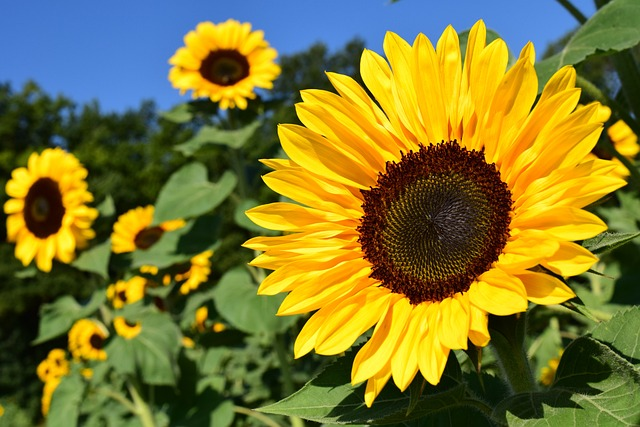
\includegraphics[width=\linewidth]{sunflower.png}
    \caption{Eingabe Bild}
    \label{fig:eingabe}
  \end{minipage}
  \hfill
  \begin{minipage}{0.47\linewidth}
    \centering
    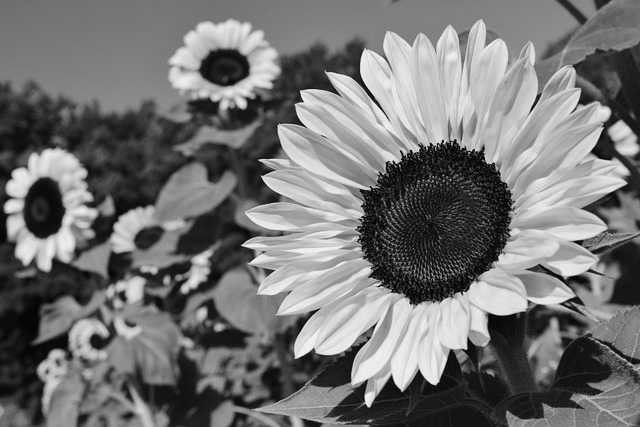
\includegraphics[width=\linewidth]{SunflowerBW.png}
    \caption{Ausgabe Bild}
    \label{fig:ausgabe}
  \end{minipage}
\end{figure}

Die Abbildungen \ref{fig:eingabe} und \ref{fig:ausgabe} repräsentieren ein Eingabebild und das entsprechende Ergebnis unserer Hauptimplementierung unter Verwendung der Standardwerte für Schwarz-, Weiß- und Mittelwerte für die Tonwertkorrektur.
Im Folgenden werden wir die ausgewählten Ansätze diskutieren, auf ihre Korrektheit prüfen und ihre Performanz analysieren.
\section{Lösungsansatz}

\subsection{Graustufen-Konvertierung}
\paragraph{Intuitiver Ansatz: Durchschnitt}

Die folgende Umrechnungsformel ist der Durchschnitt der RGB Komponenten:
 \[ D = \frac{R + G + B}{3}  \]
Die Durchschnittsmethode ist ebenfalls problematisch, da sie jeder Komponente das gleiche Gewicht zuweist.

\paragraph{Luminanz Ansatz}

Die Luminanz $Y$ dient als Maß für die Helligkeit von Bildpunkten, entsprechend der Wahrnehmung durch das menschliche Auge. Da das Auge besonders empfindlich für die Farbe Grün ist und weniger empfindlich für Blau, wird eine Gewichtung der RGB-Komponenten benötigt, um die Farbwahrnehmung des menschlichen Auges zu berücksichtigen. \cite{colorFAQ}
In unserem Kontext, bei der Arbeit mit einem PPM-Bild, das der ITU-R-Empfehlung BT.709 entspricht \cite{netpbm}, wird die folgende Umrechnungsformel gemäß Rec. 709 für die Berechnung der CIE-Luminanz aus den linearen RGB-Komponenten verwendet:
 \[Y = 0.2125R + 0.7154G + 0.0721B \cite{colorFAQ} \] 
Die ITU-R Empfehlung BT.709 definiert auch das gamma-codierte Luma $Y'$, die eine gewichtete Summe der nichtlinearen (nach Gamma-Korrektur) RGB-Komponenten entspricht, wobei gilt:
 \[Y' = 0.2126R' + 0.7152G' + 0.0722B' \cite{bt709} \] 
Die Verwendung der Luminanz bietet eine genauere Darstellung der tatsächlichen Helligkeit und eignet sich daher besser für die 8-Bit-Kodierung von Graustufen. Man muss jedoch das Bild zuvor in einen linearen RGB-Farbraum umwandeln, um den gewichteten Durchschnitt auf die linearen RGB-Komponenten anwenden zu können.
Alternativ kann jede der drei Farbkomponenten auf das berechnete Luma Y' gesetzt werden. Dies ermöglicht eine einfachere Berechnung und ist in der Praxis oft ausreichend für Graustufenbilder.
\begin{align*} 
 D &= 0.2126R' + 0.7152G' + 0.0722B' \\
 &(0.2126 + 0.7152 + 0.0722 = 1)
\end{align*}


\subsection{Tonwertkorrektur}

\subsubsection{Lineare Interpolation}
Um die drei Stützpunkten $(es, as)$, $(em, am)$ und $(ew, aw)$ zu interpolieren, wobei $es < em < ew$ gilt, können wir die lineare Interpolation anwenden.
Die linear Interpolationfunktion \( L: [0,255] \rightarrow [as,aw] \) ist wie folgt definiert:
\[
L(x) =
\begin{cases}
  as, & \text{falls } x \leq es, \\
  as + \frac{am - as}{es} \cdot (x - es), & \text{falls } es \leq x \leq em, \\
  am + \frac{aw - am}{ew - em} \cdot (x - em), & \text{falls } em \leq x \leq ew, \\
  as, & \text{falls } x \geq ew.
\end{cases}
\]

Das lineare Interpolationpolynom gewährleistet im Gegensatz zur quadratischen Interpolation, dass alle Ausgabewerte, unabhängig von den Nutzereingaben, immer innerhalb des definierten Bereichs bleiben (immer größer oder gleich $as$ und kleiner oder gleich $aw$) und somit eine zuverlässige und konsistente Interpolation gewährleistet ist.
Für eine bessere Laufzeit, haben wir uns für SIMD mit Argumenten vom Typ 8-Bit-Integer anstelle von Floats entschieden, da die genaueren Berechnungen, die durch Gleitkommazahlen erzielt werden, sowieso beim Speichern von Pixeln verloren gehen. Dies ist aufgrund der Tatsache, dass die Pixel als 8-Bit Integer dargestellt werden und die exakten Ausgabewerte nicht gespeichert werden können.

\paragraph{Bilineare Interpolation} 
Das lineare Interpolationpolynom $B: [0,255] \rightarrow [as,aw]$ ist wie folgt definiert.
\[
  B(x) =
  \begin{cases}
      as & \text{falls } x \leq es \\
      \frac{1}{2} \left(as + \frac{{(am - as) \cdot (x - es)}}{{em - es}} + as + \frac{{(aw - as) \cdot (x - es)}}{{ew - es}}\right) & \text{falls } x < em \\
      am & \text{falls } x = em \\
      \frac{1}{2} \left(am + \frac{{(aw - am) \cdot (x - em)}}{{ew - em}} + as + \frac{{(aw - as) \cdot (x - es)}}{{ew - es}}\right) & \text{falls } x > em \\
      aw & \text{falls } x \geq ew \\
  \end{cases}
\]
  

Dieser Ansatz verfolgt das Ziel, die interpolierte Funktion so zu gestalten, dass eine fließende und ausgewogene Anpassung der Graustufenwerte ermöglicht wird, insbesondere wenn die linearen Abschnitte erhebliche Unterschiede in ihren Steigungen aufweisen. Auf diese Weise wird eine konsistente Helligkeit und ein ausgewogener Kontrast im resultierenden Bild erreicht.

\subsubsection{Quadratische Interpolation}
Im Gegensatz zur linearen Interpolation kann die quadratischen Interpolationspolynome für festgelegte Werte von \((es, as)\) und \((ew, aw)\) Werte erzeugen, die außerhalb des definierten Intervalls \([as, aw]\) liegen. In diesem Fall, wird durch die Verwendung der Clamp-Funktion $aw$ zurückgegeben, wenn der Ausgabewert größer als $aw$ ist, und wird $as$  zurückgegeben, wenn der Ausgabewert kleiner als $as$ ist, damit alle Ausgabewerte innerhalb des Bereichs \([as, aw]\) bleiben. Daher ist die Funktion auf \([0,255]\)  nicht ausschließlich quadratisch und können mehrere Eingabewerte auf denselben Wert abgebildet werden.
Die Funktion \( Q: [0,255] \rightarrow [as, aw] \) ist wie folgt definiert

\[
Q(x) =
\begin{cases}
  es, & \text{if } x \leq es, \\
  \clamp{aw}{as}{s_1 \cdot x^2 + s_2 \cdot x + s_3 }, & \text{if } es < x < ew, \\
  aw, & \text{if } ew \leq x.
\end{cases}
\]

wobei die Interpolationfunktion \( I: [0,255] \rightarrow \mathbb{R} \) ist wie folgt definiert
\[ I(x) = s_1 \cdot x^2 + s_2 \cdot x + s_3 \]
Um das Interpolationspolynom zu bestimmen, wurden drei verschiedene Ansätze implementiert. Nämlich Gauß-Jordan-Algorithmus fürs Lösen des LGSs und schließlich die Evaluation des Polynoms, Lagrange-Verfahren, und Newton-Verfahren.

\paragraph{Gauß-Elimination mit Spalten-Pivotsuche} 
Das lineare Gleichungssystem für die Koeffizienten \(s_1\), \(s_2\) und \(s_3\) lautet

\[
\begin{cases}
s_3 + s_2 \cdot es + s_1 \cdot es^2 &= as, \\
s_3 + s_2 \cdot em + s_1 \cdot em^2 &= am, \\
s_3 + s_2 \cdot ew + s_1 \cdot ew^2 &= aw.\\
\end{cases}
\]

Erst muss sichergestellt, dass unser System eindeutig lösbar ist.

\begin{proof}
\[
\text{rang}\left(\begin{matrix}1 & es & es^2  \\
1 & em & em^2 \\
1 & ew & ew^2  \\
\end{matrix}\right)
=
\text{rang}\left(\begin{matrix}1 & 0 & 0 \\ 1 & em-es & em^2-es^2 \\ 1 & ew-es & ew^2-es^2\end{matrix}\right) 
\\
\] 

Da $es < em < ew$, kann keine Spalte als lineare Kombination der anderen beiden dargestellt werden und sind die drei Spalten der Matrix linear unabhängig. Diese lineare Unabhängigkeit führt dazu, dass 
\[\text{rang}\left(\begin{matrix}1 & es & es^2  \\
1 & em & em^2  \\
1 & ew & ew^2 \\
\end{matrix}\right)
=
3 \]

Es folgt dass, das Gleichungssystem immer eindeutig lösbar ist.
\end{proof}

Um Rechenfehler nicht zu verstärken, führen wir Spalten-Pivotsuche vor jedem Eliminationsschritt durch.
Wie im folgendem Algorithmus zu sehen ist.

\begin{algorithm}[H]
\caption{Gauss Jordan Verfahren}
\KwIn{$A \in \mathbb{R}^{m \times n}, b \in \mathbb{R}^{n}$}
\KwOut{$x^T = \begin{pmatrix} s_1,s_2,s_3 \end{pmatrix}$}
$h \leftarrow 1$,
$k \leftarrow 1$; \\
\While{$i \leq m$ \textbf{and} $j \leq n$} {
$pivot \leftarrow argmax (k = i ... m, abs(A[k, j]))$ \tcp*{Pivot Suche}
  \If {$A [pivot, k] = 0$} {
        $j \leftarrow j + 1$ \tcp*{Kein Pivot gefunden}
  }
  \Else{
        swap rows ($i$, pivot) \\
        \While{$k < n$} { 
          $A[i,k] \leftarrow \frac{A[i,k]}{A[i,j]}$\\
          $k \leftarrow k + 1$ \tcp*{Pivot gleich 1}
        }
        \While{$k < m$} {  
          \For{$y = 0$; $y <n; y = y + 1$} {
            $A[k, y] \leftarrow A[k, y] - A[k,j] \times A[i,y]$ \tcp*{Null Einträge}
          }
        $i \leftarrow i + 1$; \\
        $j \leftarrow j + 1$; \\
        }
  }
}
\end{algorithm}

Aus dem oben definierten Algorithmus ergibt sich die folgende Matrix
\[
\left(\begin{matrix}
1 & 0 & 0 & | & s_3 \\
0 & 1 & 0 & | & s_2  \\
0 & 0 & 1 & | & s_1
\end{matrix}\right)
\]
Mit den bestimmten Interpolationskoeffizienten können nun die Interpolationswerte berechnet werden.
Diese Implementierung handelt sich um eine naive Umsetzung des Gauß-Jordan-Algorithmus, die, wie zuvor erwähnt, stark auf der einfachen mathematischen Definition der Tonwertkorrektur basiert.
Um die Genauigkeit der folgenden Ansätze zu testen, wurde das Gauß-Jordan-Verfahren als Vergleichsimplementierung verwendet. Dies ermöglicht einen direkten Vergleich zwischen der mathematischen Definition und die anderen Algorithmen um die Korrektheit zu überprüfen.


\paragraph{Lagrange Interpolation}
Ein alternatives Algorithmus zur Bestimmung des Interpolationspolynoms, das  ein  weitverbreiteter Ansatz in der Numerik ist, besteht darin, Lagrange-Polynome zu verwenden. Hier werden Lagrange Polynomen 
der 2. Grad mit drei Stützpunkte  $(es, as)$, $(em, am)$ und $(ew, aw)$ verwendet. Die Lagrange-Polynomen sind wie folgt definiert.

\[
L_k(x) =\prod_{i:i \neq k}  \frac{(x - x_i)}{(x_k - x_i)}
\]
Als drei Basispolynomen erhalten wir in unserem Fall
\[
L_0(x) =\frac{(x - em)}{(es - em)} \cdot  \frac{(x- ew)}{(es - ew)}
\]
\[
L_1(x) =\frac{(x - es)}{(em - es)} \cdot  \frac{(x - ew)}{(em - ew)}
\]
\[
L_2(x) =\frac{(x - es)}{(ew - es)} \cdot  \frac{(x - em)}{(ew - em)}
\]
Die quadratische Interpolatisfunktion ist wie folgt definiert
\[
I(x) = \sum_{k=0}^{2} y_k \cdot L_k(x) \quad  y_i \in \{as, am, aw\}
\]

Es ist anzumerken, dass die Auswertung des Interpolationspolynoms von Daten abhängt. Dies ist für große Datensätze möglicherweise nicht besonders effizient. Es lässt sich jedoch durch eine modifizierte Alternative optimieren, nämlich die baryzentrische Lagrange Interpolation. Aufgrund der Instabilität  des Algorithmus \cite{BLagrange} wird dies jedoch weder hinsichtlich der Performanz noch der Korrektheit diskutiert.

\paragraph{Newton-Verfahren} 
Das Newton Interpolationsverfahren dient sich als alternative für die Bestimmung des Interpolationspolynoms. 
Die Newtonschen-Basispolynomen für eine quadratische Funktion mit drei Stützpunkten $(es, as)$, $(em, am)$ und $(ew, aw)$ lauten:\
\begin{align*}
   N_0(x)&=1, \\
   N_i(x)&= \prod_{j=0}^{i-1} (x-x_i) , \forall i=1,2 \quad x_1 = es, x_2 = em
\end{align*}
Die Interpolationsfunktion ist wie folgt definiert
\[
I(x) = \sum_{i=0}^{2} c_i \cdot N_i(x)
\]
Die rekursive Formel für die Newtonschen dividierten Differenzen lautet:
\begin{align*}
    c_{i,0} &= I(es) = as \\
    c_{i,k} &= \frac{c_{i+1,k-1} - c_{i,k-1}}{x_{i+k} - x_i}
\end{align*}
Diese Formel führt zu folgender Tabelle:
\begin{table}[H]
    \centering
    \begin{tabular}{|c|c|c|c|}
        \hline
        x &  0.Grad & 1.Grad & 2.Grad\\
        \hline
        es & $c_{0,0} = as $ & $c_{0,1} = \frac{am-as}{em-es}$ & $c_{0,2} = \frac{c_{1,1} - c_{0,1}}{ew-es}$\\
        \hline
        em & $c_{1,0} = am $ &$c_{1,1} = \frac{aw - am}{ew-em}$ & -- \\
        \hline
        ew & $c_{2,0} = aw $ & -- & -- \\
        \hline
    \end{tabular}
    \caption{Newtonschen dividierten Differenzen Tabelle}
    \label{tab:my_label}
\end{table}

Aus der Tabelle kann man direkt die Koeffizienten ablesen und schließlisch das Interpolationspolynom 
aufstellen.
\[
    I(x) = as + c_{0,1}\cdot(x-es)+ c_{0,2}\cdot(x-es)\cdot(x-em)
\]

\subsection{Haupt- und Vergleichsimplementierungen}
Für die Graustufen-Konvertierung bzw. die Tonwertkorrektur wurden entsprechend den Luminanz Ansatz bzw. die quadratische Interpolation mittels Gauss-Jordan-Algorithmus ausgewählt. Anschließend stellen die beiden Ansätze durch SIMD-Optimierungen die Kerne unserer Hauptimplementierung. \
Zusätzlich wurden drei weitere Versionen definiert:
\begin{itemize}
    \item Version 1: Diese entspricht der Algorithmik der Hauptimplementierung, wurde jedoch sequenziell implementiert. Da diese Version einfach die mathematische Definition der Tonwertkorrektur umsetzt, dient sie als Vergleichsimplementierung.
    \item Version 2: Hierbei handelt es sich um eine SIMD-Implementierung des Newton-Verfahrens, die eine vergleichbare Laufzeit zur Hauptimplementierung aufweist, wie später in der Performanzanalyse gezeigt wird.
    \item Version 3: Diese ist eine SIMD-Implementierung der linearen Interpolation. Je nach den nutzerspezifizierten Eingabewerten der Pixel könnte diese Version möglicherweise besser geeignet sein.
\end{itemize}


\section{Korrektheit}
In diesem Abschnitt wird die Korrektheit und Genauigkeit unserer Implementierung überprüft.

\subsection{Genauigkeit}
Es wird erstens sichergestellt, dass unsere Implementierung unter spezifischen Szenarien die erwarteten Ausgaben liefert.\\
Wir stellen sicher, dass das implementierende Gaußsche Verfahren zur Lösung des linearen Gleichungssystems genaue Ergebnisse liefert. Es ist besonders wichtig, diesen Ansatz auf Genauigkeit zu überprüfen, da die Methode schlicht nah der mathematischen Definition ist. Sie dient daher als Ausgangspunkt zur Überprüfung der Korrektheit der nachfolgenden Ansätze.

\subsection{Korrektheit}

Im ersten Abschnitt wird verifiziert, dass die SIMD Implementierungen korrekt funktionieren, indem die Ausgabe-Pixel-Arrays der SIMD- und SISD- Implementierungen direkt miteinander verglichen werden. Diese Methode stellt eine robuste Strategie dar, um sicherzustellen, dass die SIMD Implementierung keine Kompromisse bei der Genauigkeit mit sich bringt. \\
Der zweite Teil gewährleistet, dass die implementierenden quadratischen Algorithmen, nämlich das Newton-Verfahren und das Lagrange-Verfahren, die korrekten Ergebnisse liefern. Aus dem Grund, dass das Interpolationspolynom stets eindeutig ist, stellt der Vergleich der Ausgaben dieser Methoden eine zuverlässige Strategie dar, um die Korrektheit unserer Implementierungen zu gewährleisten.


\section{Performanzanalyse}
In diesem Abschnitt soll die Performanz der einzelnen Lösungsansätze analysiert und bewertet werden. Als Messumgebung wurde das Programm mit GCC 11.4.0 und Optimierungsstufe 3 auf einem System mit einem Intel i5-8250U Prozessor, 1.60 GHz, 4 GB Arbeitsspeicher, Xubuntu 22.04 und Linux Kernel 6.5 kompiliert. \\
Die Messungen in den folgenden Abschnitten werden in Millisekunden pro Anzahl der Pixel angegeben, um ein konsistentes Maß über verschiedene Dateigrößen hinweg zu gewährleisten. Die Berechnungen wurden mit Bildern verschiedener Auflösungen (63$\times$63,  1280$\times$853, usw.) jeweils 100 Mal für die kleinen, 50 Mal für die mittlen und 20 Mal für die größen durchgeführt. Anschließend wird der Durchschnittswert berechnet und angegeben. \\ 
Es ist wichtig zu erwähnen, dass nur die Laufzeit des angegebenen Algorithmus berücksichtigt wird. Das Einlesen des Eingangsbildes bzw. die Generierung des neuen Bildes ist ausgeschlossen.

\subsection{Quadratic Interpolations-Algorithmen}
In unserem Projekt wurden drei verschiedene Ansätze zur Realisierung der quadratischen Interpolation verwendet. Wir werden im nächsten die drei Algorithmen, nämlich Gauß-Jordan-Verfahren, Lagrange Interpolation und Newton Interpolation, auf Laufzeit vergleichen. 
\begin{figure}[H]
  \centering
  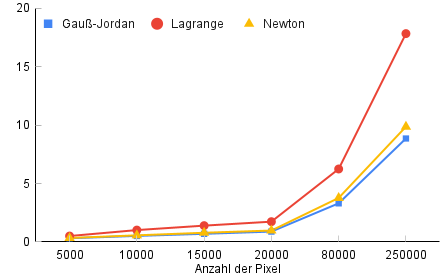
\includegraphics[width=0.65\textwidth]{quadAlg.png}
  \caption{Quadratische Interpolations-Algorithmen}
  \label{fig:quadalg}
\end{figure}
Wie oben gezeigt ist die Lagrange-Interpolation die zeitaufwendigste Alternative. Dies liegt daran, dass das Ergebnis kontinuierlich von den Daten abhängt, was bedeutet, dass das Auswerten jeder Interpolationspolynome $O(n^2)$ flops erfordert.
Die Newton-Interpolation hingegen ist deutlich effizienter, was sich besonders bei einer relativ großen Anzahl von über $10^4$ Pixel bemerkbar macht. Das Verfahren erfordert ungefähr $n^2$ Subtraktionen und $\frac{n^2}{2}$ Divisionen für das Aufstellen der Differenzenquotienten-Tabelle, sowie für jedes Auswerten von  Interpolationspolynom $n$ flops aufgrund verschachtelter Multiplikationen. Dadurch ergibt sich eine zeitliche Komplexität, die deutlich geringer ist als die der Lagrange-Interpolation. \\
Auffällig ist, dass das Lösen des Systems mittels Gauß-Jordan-Verfahrens eine effiziente Alternative darstellt, was nicht wie zunächst vermutet war. Das Verfahren wird oft als ineffizient und numerisch unzuverlässig angesehen. Es erfordert $\frac{n^3}{2}$ Multiplikationen und Divisionen für das Lösen von Gleichungssystemen. In unserem Fall ist die Matrix 3x4 groß und bereits für die Pivotsuche aussortiert, weshalb keine Pivotisierung stattfindet. Dadurch ergibt sich, dass das Aufstellen des Polynoms ungefähr 13 flops erfordert, im Gegensatz zu den 15, die für das Aufstellen der Differenzenquotienten-Tabelle bei der Newton-Interpolation benötigt werden. Zusätzlich erfordert das Auswerten bei der Gauß-Jordan-Verfahren keine Substitution, was zu einer effizienteren Auswertung des resultierenden Polynoms im Vergleich zur Newton-Interpolation führt.
Dies ist für eine relativ kleine Anzahl an Pixel kaum spürbar, wird jedoch ab etwa $10^6$ Pixeln bemerkbar.


\subsection{Weitere Optimierungen}

\subsection*{Gauss-Jordan-Verfahren}
Aus dem letzten Abschnitt ergibt sich die Auswahl eines Algorithmus für die quadratische Interpolation. Im folgenden Abschnitt werden wir diesen ausgewählten Algorithmus weiter optimieren, indem wir Look-Up-Tabellen verwenden und die Prozessor Vektoren durch SIMD (Single Instruction, Multiple Data) optimal nutzen.
\begin{figure}[H]
  \centering
  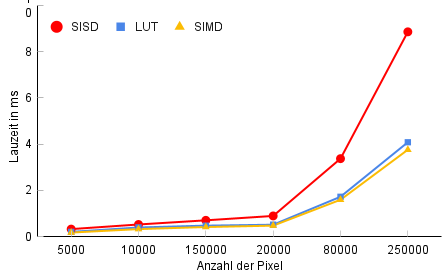
\includegraphics[width=0.65\textwidth]{quadOpt.png}
  \caption{Gaus-Jordan-Verfahren Versionen}
  \label{fig:quadopt}
\end{figure}
Die SIMD Implementierung (Abbildung \ref{fig:quadopt}, gelbe Linie) erzielt in Relation zu den SISD einen Speedup von circa 3. Dies geschieht dadurch, dass die Vektorisierung vier Farbkanäle gleichzeitig verarbeitet, im Gegensatz zu der vollständigen sequentiellen Berechnung. Theoretisch wäre der maximale Speedup von 4, was jedoch vom gemessenen Speedup von 3 abweicht, was auf den durch das Laden und Aufbereiten der Vektoren entstehenden Overhead zurückzuführen ist. Bei der Vektorisierung wurden 32-Bit-Floats verwendet. Alternativ könnten die Berechnungen mit 16-Bit-Integern durchgeführt werden, was zu einem Genauigkeitsverlust führt. Dies ist vor allem dann relevant, wenn die Stützpunkte der Interpolation deutlich von den Standardwerten abweichen. Der Trade-off zwischen Genauigkeit und einem theoretischen Speedup von 8 wurde als nicht gerechtfertigt erachtet, da die Stützpunkte von den Eingabewerten abhängen und dadurch stark variieren können.\\ 
Die Look-up-Tabelle (Abbildung \ref{fig:quadopt}, blaue Linie) weicht in Performanz nicht signifikant von der SIMD-Alternative ab und ist für kleinere Eingaben kaum bemerkbar. Die Tabelle wird als ”On-the-fly”  LUT implementiert. Zuerst wird die Tabelle während des ersten Auftretens verschiedener Eingabewerte aufgefüllt und anschließend nur noch gelesen. Da die Tabelle maximal 256 Bytes groß ist, wird sie in meisten Fälle  gecacht, was im Vergleich einen Kostengünstigen Zugriff ermöglicht. Obwohl die erste Phase, das Ausfüllen der Look-Up-Tabelle, aufgrund von Cache-Effekten kostenintensiv ist, wird dies fast immer ausgeglichen, da in der Regel mehr als 256 Pixel große Bilder auftreten und dabei fast immer Einsparungen erzielt werden. 

\subsection*{Graustufen-Konvertierung}
Wie oben beschrieben, eignet sich auch die Graustufen-Konvertierung gut für die Vektorisierung. Im folgenden Diagramm wird der Unterschied in der Laufzeit zwischen der vollständigen sequentiellen Berechnung und der SIMD-Alternative dargestellt.
\begin{figure}[H]
  \centering
  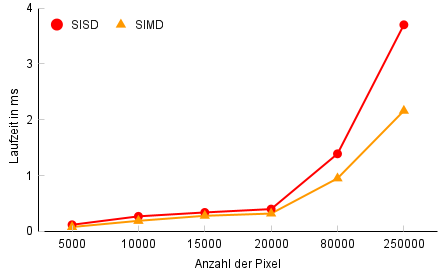
\includegraphics[width=0.65\textwidth]{graySDMD.png}
  \caption{Graustufen-Konvertierung Versionen} 
  \label{fig:graysimd}
\end{figure}
Die SIMD-Implementierung zeigt lediglich einen Speedup von 1,5 im Vergleich zu den SISD-Implementierungen. Dies liegt teilweise wiederum am entstehenden Overhead beim Laden und Aufbereiten der Vektoren. Darüber hinaus hat der GCC-Compiler ab Optimierungsstufe 3 die SISD-Alternative stark optimiert, indem er Strength Reduction und Register-Allokation durchgeführt hat. Dadurch wurde die Laufzeit der sequentiellen Bearbeitung deutlich verringert.

\subsection{Hauptimplementierung}
Schließlich wurden die Laufzeiten der Hauptimplementierung und der Vergleichsimplementierung gemessen. Dazu wurde die Gesamtzeit für die Graustufenkonvertierung und die Tonwertkorrektur für beide Varianten gemessen und in das folgende Diagramm eingetragen.
\begin{figure}[H]
  \centering
  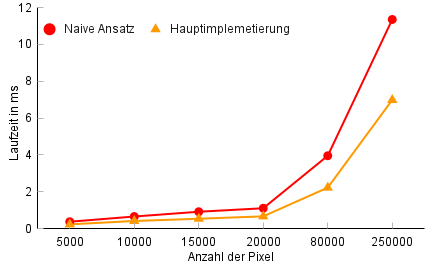
\includegraphics[width=0.65\textwidth]{mainComp.png}
  \caption{Haupt- und Vergleichsimplementierung} 
  \label{fig:mainComp}
\end{figure}
Wie in den vorherigen Abschnitten besprochen, hat die Wahl eines effizienten Algorithmus für die quadratische Interpolation sowie die SIMD-Optimierung der beiden Kerne des gesamten Algorithmus belohnt und einen Speedup von 2 für das gesamte Vorgehen erzielt.

\section{Zusammenfassung und Ausblick}
In diesem Projekt haben wir die Tonwertkorrektur für PPM (P6) Bilder durchgeführt und dabei verschiedene Algorithmen und Optimierungen eingesetzt. Zunächst wurde die Graustufenkonvertierung durch den Luminanz Ansatz realisiert und entsprechend mit SIMD optimiert. Anschließend wurden verschiedene Algorithmen zur Tonwertkorrektur verglichen und bewertet. Diese Algorithmen lassen sich in zwei Kategorien einteilen: lineare Interpolation und quadratische Interpolation. Für die Hauptimplementierung wurde das Gauß-Jordan-Verfahren ausgewählt und entsprechend mit SIMD optimiert. 
Weitere Optimierungen sind möglich. Durch die hohe Parallelität moderner Rechenkerne lässt sich Multithreading effektiv nutzen.
 Zudem kann die Implementierung angepasst werden, um weitere Stützpunkte einzulesen und Tonwertkorrekturen mit höhergradigen Interpolationspolynomen zu berechnen. Hierfür kann dies weiter optimiert werden und die Horner'sche Methode anstelle der naiven Auswertung des Polynoms verwendet werden.	
\bibliographystyle{plain}
\bibliography{Ausarbeitung}{}

\end{document}